% PointWorld presenter deck. CS 2883R, Wed 18 Nov 2026. Juntang Wang and Vivian Hui.
% Numbers checked against arXiv 2601.03782v1; each frame comment names its source.
% Rules: one claim per frame, at most 3 bullets, no bullet restating its own figure;
% teal marks PointWorld or the one number to carry; l2 errors are in metres, so 0.001 is
% 1 mm; zero-shot means no demos and no finetuning, not no human input (masks and targets
% are drawn by hand); equations, full tables and protocol details live in the backup.
% The presenter speaks as the first author (course guidelines): our critique lives in the
% Discussion questions and the "Our reading" backup, for the reviewer and red-team roles.
% 15:00 for two speakers, about 13:45 budgeted. Handoff after planning.
% If long, cut "Why gripper points" first. LAPA deck: git tag lapa-final.
% Build: latexmk -pdf main.tex
\documentclass[aspectratio=169,12pt]{beamer}
\usetheme[progressbar=none, numbering=counter]{moloch}

\usepackage[sfdefault,light]{FiraSans}
\usepackage[T1]{fontenc}
\usepackage{tikz}
\usepackage{booktabs}
\usepackage{multicol}
\usepackage[authoryear, round]{natbib}
\definecolor{cite}{HTML}{1F5FBF}  % citations and URLs: blue, clickable
\hypersetup{colorlinks=true, citecolor=cite, urlcolor=cite, linkcolor=.}
\renewcommand{\bibsection}{}                          % the frame title is enough
\bibliographystyle{plainnat}
% Beamer 3.77 + current hyperref leave natbib's \hyper@natlinkbreak empty, which drops the
% ", " in (Author et al., 2024) and the " (" in Author et al. (2024). Restore hyperref's definition.
\makeatletter
\AddToHook{begindocument/end}{%
  \def\hyper@natlinkbreak#1#2{\hyper@linkend#1\hyper@linkstart{cite}{cite.#2}}}
\makeatother

\definecolor{ink}{HTML}{222222}
\definecolor{mute}{HTML}{8a8a8a}
\definecolor{pw}{HTML}{12807A}       % PointWorld rows and accents
\definecolor{crimson}{HTML}{A51C30}  % Harvard; title slide only

\setbeamercolor{normal text}{fg=ink, bg=white}
\setbeamercolor{frametitle}{fg=ink, bg=white}
\setbeamercolor{page number in head/foot}{fg=mute}
\setbeamertemplate{itemize items}{\color{pw}--}
\setlength{\leftmargini}{1.1em}

\newcommand{\src}[1]{{\scriptsize\color{mute}\citep{#1}}}
\newcommand{\paperfig}[3]{%
  \begin{tikzpicture}[baseline=(f.south)]
    \node[inner sep=0pt] (f) {\includegraphics[#1]{#2}};
    \node[anchor=north east, inner sep=1pt, font=\tiny, text=mute] at (f.south east)
      {\citet{huang2026pointworld}, #3};
  \end{tikzpicture}}
\newcommand{\credit}[1]{\par\hfill{\tiny\color{mute}\citet{huang2026pointworld}, #1}\par}
\newcommand{\pw}[1]{{\color{pw}#1}}
\newcommand{\colhead}[2]{\begin{minipage}[t][1.5cm]{\linewidth}\raggedright
  {\small\bfseries #1}\\\src{#2}\end{minipage}\\}
\newenvironment{notes}[1][\linewidth]
  {\begin{minipage}{#1}\footnotesize\begin{itemize}\setlength{\itemsep}{2pt}}
  {\end{itemize}\end{minipage}}

\begin{document}

% 0. Title  0:15
\begin{frame}[plain]
  \vfill
  {\LARGE\bfseries PointWorld: Scaling 3D World Models\\[2pt]
    for In-The-Wild Robotic Manipulation}\\[6pt]

  {\scriptsize\color{mute} Wenlong Huang, Yu-Wei Chao, Arsalan Mousavian, Ming-Yu Liu,
    Dieter Fox, Kaichun Mo, Li Fei-Fei.\\ Stanford, NVIDIA.\
    CVPR 2026. arXiv 2601.03782. Code, data and checkpoints: github.com/NVlabs/PointWorld}

      \textcolor{crimson}{\rule{\textwidth}{0.8pt}}\\[8pt]
  Juntang Wang $\cdot$ Vivian Hui\\[2pt]
  \vfill
\end{frame}

%% ---- Part A: problem and method, about 7:15 ----

% 1. Problem  1:00  (S1, Fig. 1, abstract)
\begin{frame}{Problem}
  \centering
  \paperfig{height=3.9cm}{figs/fig1_teaser.pdf}{Fig.~1}
  \vfill
  \begin{notes}[0.9\linewidth]
    \item A \textbf{world model} for manipulation: given what the robot sees and what it
      intends to do, predict how the scene will move
    \item The goal here: from one RGB-D image of an unseen room, in 3D, for more than one robot
    \item \pw{Represent the scene and the robot's action the same way, as moving 3D points,
      and train one model on 2M trajectories}
  \end{notes}
  \vfill
\end{frame}

% 2. Before PointWorld  0:45  (S1, S2; seconds-long inference from S3.1)
\begin{frame}{Before PointWorld}
  \begin{columns}[t]
    \column{0.31\textwidth}
      \colhead{Physics simulators}{todorov2012mujoco}
      \footnotesize
      \begin{itemize}
        \item Accurate once the scene is modelled: meshes, masses, materials
        \item That modelling is per scene, and the sim-to-real gap remains
      \end{itemize}
    \column{0.31\textwidth}
      \colhead{Learned particle dynamics}{li2018particle, ai2025review}
      \footnotesize
      \begin{itemize}
        \item Learn from interaction, often as graphs over particles (GBND)
        \item Usually scene-specific, with full observability, object or material priors
      \end{itemize}
    \column{0.31\textwidth}
      \colhead{Video world models}{brooks2024sora, agarwal2025cosmos, assran2025vjepa2}
      \footnotesize
      \begin{itemize}
        \item Trained at scale and look real, but physics is often off
        \item Actions come in as text or robot commands, not geometry; seconds per prediction
      \end{itemize}
  \end{columns}
  \vspace{14pt}
  \centering\footnotesize
  \pw{PointWorld keeps the particle view, and scales it the way video models scale}
\end{frame}

% 3. Method  1:30  (S3.1, Fig. 2; 300-500 gripper points from S5.2)
\begin{frame}{Method}
  \begin{columns}[c]
    \column{0.40\textwidth}
      \centering
      \paperfig{height=5.0cm}{figs/fig2_overview.pdf}{Fig.~2}
    \column{0.58\textwidth}
      \footnotesize
      \begin{itemize}\setlength{\itemsep}{5pt}
        \item \textbf{State}: the RGB-D image back-projected to a point cloud, robot pixels
          removed. Each point carries frozen DINOv3 features \src{simeoni2025dinov3}
        \item \textbf{Action}: 300 to 500 points per gripper, placed by forward kinematics at
          each of the next 10 steps and tagged with a time embedding. A Franka and a
          two-armed humanoid are described the same way
        \item \textbf{Model}: PTv3 \src{wu2023ptv3} reads scene and robot points as one
          cloud; a shared head gives every scene point's displacement at all 10 steps,
          0.1\,s apart, in one pass
      \end{itemize}
      \vspace{4pt}
      {\footnotesize\pw{State and action live in one space: 3D points}\par}
  \end{columns}
\end{frame}

% 4. What the target asks for  0:45  (Fig. 3, S1; DINOv3 as objectness prior, S5.1)
\begin{frame}{What one target asks for}
  \centering
  \paperfig{width=0.94\linewidth}{figs/fig3_supervision.pdf}{Fig.~3}
  \vfill
  \begin{notes}[0.94\linewidth]
    \item To predict where every point goes, the model has to work out what is an object,
      what is soft or hinged, the hidden back of a box, and gravity
    \item \pw{Training gives no object masks, material labels or physics engine: only the
      point displacements, helped by frozen DINOv3 features}
  \end{notes}
  \vfill
\end{frame}

% 5. Training loss  1:00  (Eq. 1, S3.1, Fig. 4; 1-5% from S5.1; full form in backup)
\begin{frame}{Training loss}
  \centering
  \paperfig{width=0.86\linewidth, trim=0 0 0 129, clip}{figs/fig4_weighting.pdf}{Fig.~4, bottom row}
  \vspace{2pt}
  {\small $\displaystyle \mathcal L = \tfrac12 \sum_{k,i} w_{k,i}
    \Big( \rho_\delta\big(\hat P_{t+k,i} - P_{t+k,i}\big)\, e^{-s_{k,i}} + s_{k,i} \Big)$\par}
  \vspace{2pt}
  \begin{notes}[0.86\linewidth]
    \item Only 1--5\% of points move. $w$ shifts the loss onto them, using the true
      displacement
    \item Real labels are noisy. The model predicts its own log-variance $s$ per point,
      which down-weights bad labels, and $\rho_\delta$ is a Huber loss
    \item \pw{$s$ also picks up physics: it is largest along the edge of a dropped cloth}
  \end{notes}
\end{frame}

% 6. Data  1:15  (S4, Fig. 5)
\begin{frame}{Data: re-annotating DROID in 3D}
  \centering
  \paperfig{height=3.3cm}{figs/fig5a_annotation.pdf}{Fig.~5, top}
  \vfill
  \begin{notes}[0.86\linewidth]
    \item DROID \src{khazatsky2024droid}: real teleoperation in hundreds of scenes, but its
      sensor depth and camera poses are off
    \item Three steps: depth from FoundationStereo \src{wen2025foundationstereo}, poses
      from VGGT \src{wang2025vggt} refined against the robot mesh, CoTracker3
      \src{karaev2025cotracker3} tracks lifted to 3D
    \item \pw{Over 60\% of DROID survives, about 200 hours}. With BEHAVIOR-1K simulation
      \src{li2024behavior}, the total is about 2M trajectories, 500 hours
  \end{notes}
  \vfill
\end{frame}

% 7. Planning  0:45  (S3.2, Eq. 2, App. real-robot details)
\begin{frame}{Planning with the model}
  \small
  \[
    \min_{E_{0:T}} \sum_{k=1}^{T} c_{\text{task}}(s_k) + c_{\text{ctrl}}(E_k)
    \quad \text{s.t.}\quad s_{1:T} = F_\theta(s_0, a_{1:T})
  \]
  {\scriptsize\color{mute} $E_k$: end-effector pose\, $\cdot$\, $s_k$: predicted scene
    points\, $\cdot$\, $a_k$: gripper points placed at $E_k$\par}
  \vspace{8pt}
  \begin{notes}[0.9\linewidth]
    \item MPPI \src{williams2017mppi}: perturb a gripper path, roll each one out through
      PointWorld, average the paths weighted by how low their cost is
    \item The cost: move the points of a hand-drawn object mask to hand-placed targets,
      plus a mild pull toward the object, path length and reachability
    \item \pw{One image in, a plan 30 steps (3\,s) long out, in a few seconds}
  \end{notes}
\end{frame}

%% ==== HANDOFF: second speaker starts here (split to agree with Vivian) ====

%% ---- Part B: evidence, about 6:30 ----

% 8. How it is scored  0:45  (S4 evaluation protocol, Fig. 6 top two rows)
\begin{frame}{How it is scored}
  \centering
  \paperfig{width=0.92\linewidth, trim=16 485 0 0, clip}{figs/fig6_rollouts.pdf}{Fig.~6, top two rows}
  \vfill
  \begin{notes}[0.92\linewidth]
    \item \textbf{$\ell_2$ mover}: mean distance, in metres, between predicted and true
      positions of the points that move, over the 1\,s horizon
    \item On DROID, points count only where a separate model, trained on the test split, is
      confident (\S4: the top 80\%)
    \item \pw{0.001 is one millimetre. Read every difference that follows in mm}
  \end{notes}
  \vfill
\end{frame}

% 9. Roadmap  1:00  (Fig. 7, S5.1)
\begin{frame}{Recipe: what each change bought}
  \begin{columns}[c]
    \column{0.40\textwidth}
      \centering
      \paperfig{height=6.0cm}{figs/fig7_roadmap.pdf}{Fig.~7}
    \column{0.58\textwidth}
      \footnotesize
      \begin{itemize}\setlength{\itemsep}{5pt}
        \item Swapping the graph network (GBND) for PTv3 is the biggest single step:
          0.0386 to 0.0348
        \item The loss and DINO image features add 1.7\,mm; scaling PTv3 from 50M to 1B
          parameters adds 1.9\,mm
        \item \pw{0.0386 to 0.0312 overall: 7.4\,mm, or 19\% less error on moving points}
      \end{itemize}
      \vspace{4pt}
      {\scriptsize\color{mute} Each bar adds one change to the bar above it. Hatched bars
        were tried and not kept.\par}
  \end{columns}
\end{frame}

% 10. Scaling  0:45  (Fig. 9, S5.2 scaling paragraph; Tab. 1 for memory and latency)
\begin{frame}{Scaling}
  \begin{columns}[c]
    \column{0.42\textwidth}
      \centering
      \paperfig{height=4.7cm}{figs/fig9_scaling.pdf}{Fig.~9}
    \column{0.56\textwidth}
      \footnotesize
      \begin{itemize}\setlength{\itemsep}{5pt}
        \item Error falls roughly log-linearly with data, from 5\% to 100\% of DROID, and
          with model size, from 50M to 1B parameters
        \item PTv3 makes the model axis affordable: 957 times GBND's parameters for 4.3
          times the memory, about 0.12\,s per pass at 1B (Tab.~1)
        \item \pw{Predictable gains from more data and capacity, as in language and vision}
      \end{itemize}
      \vspace{4pt}
      {\scriptsize\color{mute} One axis at a time, on DROID. All nine backbones in the
        backup.\par}
  \end{columns}
\end{frame}

% 11. Why gripper points  0:45  (Fig. 11, S5.2) -- first to cut if running long
\begin{frame}{Why gripper points?}
  \begin{columns}[c]
    \column{0.44\textwidth}
      \centering
      \paperfig{height=4.4cm}{figs/fig11_action.pdf}{Fig.~11}
    \column{0.54\textwidth}
      \footnotesize
      \begin{itemize}\setlength{\itemsep}{5pt}
        \item Robot as points on its grippers only, against points on the whole body (two
          densities), end-effector pose, or joint positions
        \item Lowest error on both real (DROID) and simulated (B1K) data. On real data,
          whole-body points do worse than a plain pose; the authors' reading: too many robot
          points drown the few moving scene points
        \item \pw{Gripper points keep the contact geometry and stay the same format for
          both robots}
      \end{itemize}
      \vspace{4pt}
      {\scriptsize\color{mute} All variants are trained on DROID and B1K together. The
        paper does not say what the markers above the bars are.\par}
  \end{columns}
\end{frame}

% 12. Transfer to a new lab  1:00  (Tab. 2 held-out columns, S5.3; finetuning = 1/20
%     of the iterations)
\begin{frame}{Does it transfer to a new lab?}
  \centering\small
  \setlength{\tabcolsep}{9pt}
  \begin{tabular}{@{}lcccc@{}}
    \toprule
    pretrained on & DROID & BEHAVIOR-1K & \pw{both} & specialist (H only) \\
    \midrule
    zero-shot & 0.0305 & 0.0531 & \pw{0.0300} & 0.0293 \\
    finetuned & \textbf{0.0271} & 0.0299 & \pw{\textbf{0.0272}} & 0.0293 \\
    \bottomrule
  \end{tabular}
  \credit{Tab.~2, held-out columns, $\ell_2$ mover; in- and cross-domain columns in the
    backup}
  \vfill
  \begin{notes}[0.9\linewidth]
    \item H: one DROID lab held out of pretraining. The specialist trains on that lab alone
    \item Zero-shot, real-plus-sim pretraining comes within 0.7\,mm of the specialist.
      \pw{Finetuned with 1/20 of the training steps, it beats the specialist by 2.1\,mm}
    \item Simulation alone does not transfer zero-shot, but finetuning brings it close to
      the specialist
  \end{notes}
  \vfill
\end{frame}

% 13. Real robot  1:15  (Fig. 8, S5.4, App. real-robot details)
\begin{frame}{Results: real robot, zero-shot}
  \centering
  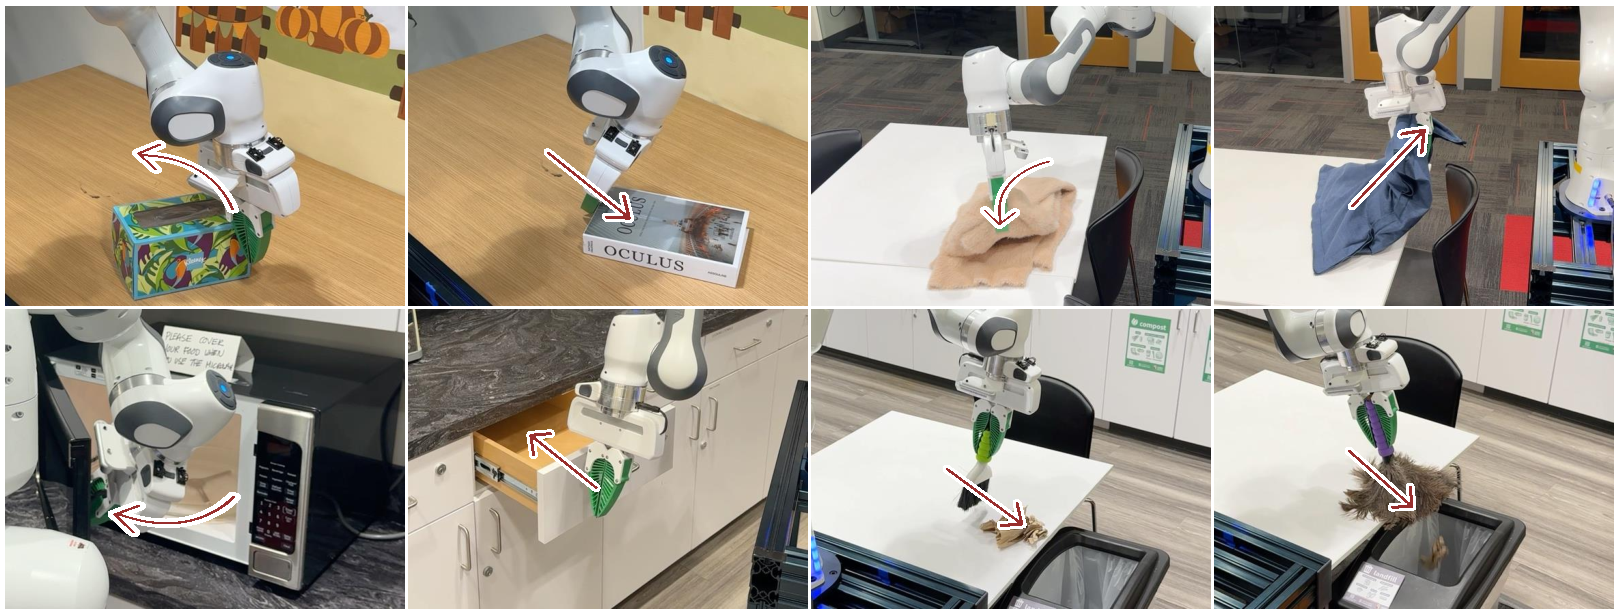
\includegraphics[height=2.5cm]{figs/fig8b_tasks.pdf}\\[1pt]
  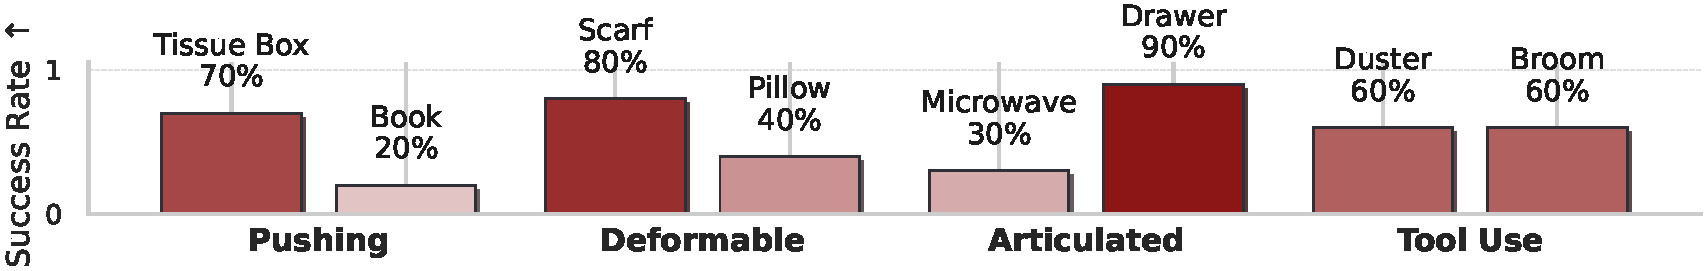
\includegraphics[width=0.66\linewidth]{figs/fig8a_success.pdf}
  \credit{Fig.~8}
  \vspace{2pt}
  \begin{notes}[0.9\linewidth]
    \item 8 tasks, 10 trials each, one camera, and a fin-ray gripper the model never saw
      in training. No demos, no finetuning
    \item \pw{56\% overall (45 of 80)}, from 2 of 10 pushing a book to 9 of 10 closing a
      drawer
    \item Each plan runs without replanning; the deformable and tool tasks start with the object
      grasped. Videos: \href{https://point-world.github.io}{point-world.github.io}
  \end{notes}
\end{frame}

% 14. Limitations  0:30  (App. "Extended Discussions on Limitations")
\begin{frame}{Limitations}
  \vfill
  \begin{columns}
    \column{0.86\textwidth}
      {\small\bfseries Stated by the authors} {\scriptsize\color{mute}(Appendix)}
      \vspace{4pt}
      \begin{itemize}\setlength{\itemsep}{6pt}
        \item One still frame in, so the scene must start at rest: no velocities
        \item Task costs are drawn by hand: object masks and target points
        \item The robot is assumed rigid and to follow its planned path exactly
      \end{itemize}
  \end{columns}
  \vfill
\end{frame}

% 15. Takeaway  0:30
\begin{frame}{Takeaway}
  \vfill
  \begin{columns}
    \column{0.88\textwidth}
      \begin{itemize}\setlength{\itemsep}{10pt}
        \item \pw{One 3D world model for more than one robot: scene and action as moving
          points, trained on 2M real and simulated trajectories}
        \item Each piece of the recipe lowers the error, and more data and parameters keep
          helping at a predictable rate
        \item From a single image it plans real pushing, cloth, hinge and tool tasks
          zero-shot; code, data and checkpoints are public
      \end{itemize}
  \end{columns}
  \vfill
\end{frame}

% 16. Discussion  -- the 15 minutes end here; call on the roles in the agreed order.
%     Each question hands a thread to a role (reviewer, red team, researcher).
\begin{frame}{Discussion}
  \begin{itemize}\setlength{\itemsep}{6pt}
    \item The robot results report no baseline and never replan. What comparison would
      show that 56\% is good?
    \item On real data a plain end-effector pose comes close to gripper points. Is the
      point action essential, or mainly a way to mix robots?
    \item The model sees one frozen frame, and moving points are still off by about
      3\,cm. Which tasks does that rule out?
  \end{itemize}
\end{frame}

%% ---- backup ----
\appendix

% Our critique, kept out of the main talk (presenter = first author). Sources: S4, S5.2,
% S5.3, S5.4, App. DROID evaluation protocol, App. real-robot details.
\begin{frame}{Backup: our reading}
  \footnotesize
  \begin{itemize}\setlength{\itemsep}{5pt}
    \item \textbf{Robot}: 8 tasks $\times$ 10 trials, no baseline success rate, no
      replanning, deformable and tool tasks start pre-grasped. 56\% cannot yet be ranked
      against a policy or another model
    \item \textbf{Metric}: real-data gaps are a few mm, scored on points an expert model
      trusts. \S4 says it keeps the top 80\%; the appendix thresholds ``at the 0.8
      quantile'' and drops the points below, which reads as the top 20\%
    \item \textbf{Transfer}: zero-shot on a held-out lab is 0.7\,mm behind the specialist;
      the clear wins need finetuning
    \item \textbf{Small inconsistencies}: GBND is 0.0390 in Tab.~1 and 0.0386 in Fig.~7.
      Fig.~11's legend gives whole-body variants of 500 and 3000 points; \S5.2 gives ``the
      same number of points'' and 2000
  \end{itemize}
\end{frame}

% Eq. 1 and the movement weight, S3.1
\begin{frame}{Backup: training objective}
  \small
  \[
    \tfrac12 \sum_{k,i}^{H, N_S}
    \underbrace{w_{k,i}}_{\text{movement}}
    \Big( \underbrace{\rho_\delta\big(\hat P_{t+k,i} - P_{t+k,i}\big)}_{\text{Huber on 3D residual}}
    \underbrace{e^{-s_{k,i}}}_{\text{uncertainty weight}}
    + \underbrace{s_{k,i}}_{\text{regularizer}} \Big)
    \tag{1}
  \]
  \[
    m_{k,i} = \sigma\big(\kappa(\delta_{k,i} - \tau)\big), \qquad
    w_{k,i} = m_{k,i} \Big/ \textstyle\sum_{k,i} m_{k,i}
  \]
  \credit{\S3.1}
  \vfill
  \begin{notes}
    \item $\delta_{k,i}$: length of point $i$'s true displacement at step $k$; $\tau$ a
      threshold, $\kappa$ a temperature
    \item Points the 2D tracker marks as occluded get no loss at all
    \item Aleatoric uncertainty, the same device VGGT uses \src{wang2025vggt}: the model may
      say ``unsure'', at the price of the $s$ term
  \end{notes}
\end{frame}

% App. real-robot details
\begin{frame}{Backup: planning and robot protocol}
  \footnotesize
  \begin{columns}[t]
    \column{0.48\textwidth}
      {\small\bfseries Planner}
      \begin{itemize}\setlength{\itemsep}{2pt}
        \item MPPI around a zero nominal, cubic-spline noise (4 knots), $\sigma$ from 0.05
          to 0.50
        \item 256 samples, temperature $\beta = 0.05$, EMA 0.9, 20 iterations
        \item 30 steps ahead, in 3 chunked passes; no replanning in this work
      \end{itemize}
    \column{0.48\textwidth}
      {\small\bfseries Robot}
      \begin{itemize}\setlength{\itemsep}{2pt}
        \item 7-DoF Franka on a wheeled base, 3D-printed fin-ray gripper (training saw
          Robotiq and Galaxea R1 Pro grippers)
        \item One RealSense D435; depth from its stereo IR pair via FoundationStereo
        \item Masks from SAM~2 \src{ravi2024sam2}, targets placed in a GUI; failures include
          plans judged unsafe to run
      \end{itemize}
  \end{columns}
  \vspace{4pt}\credit{Appendix, real-robot experiment details}
\end{frame}

\begin{frame}{Backup: all backbones}
  \centering\small
  \setlength{\tabcolsep}{5pt}
  \begin{tabular}{@{}lrrrrrr@{}}
    \toprule
    & params & memory & FLOPs & latency (ms) & $\ell_2$ mover & $\ell_2$ static \\
    \midrule
    GBND \src{ai2025review} & 1.00$\times$ & 1.00$\times$ & 1.00$\times$ & 13.46 & 0.0390 & 0.0066 \\
    PointNet & 1.03$\times$ & 0.34$\times$ & 0.04$\times$ & 5.93 & 0.0369 & 0.0084 \\
    PointNet++ & 1.07$\times$ & 0.67$\times$ & 0.06$\times$ & 327.08 & 0.0368 & 0.0073 \\
    SparseConv & 33.31$\times$ & 7.18$\times$ & 1.32$\times$ & 17.70 & 0.0396 & 0.0076 \\
    Transformer & 41.06$\times$ & 0.31$\times$ & 3.38$\times$ & 30.43 & 0.0339 & 0.0071 \\
    \pw{PTv3-50M} & 49.14$\times$ & 0.30$\times$ & 0.34$\times$ & 59.60 & 0.0331 & 0.0067 \\
    \pw{PTv3-132M} & 127.22$\times$ & 0.69$\times$ & 1.04$\times$ & 69.60 & 0.0324 & 0.0061 \\
    \pw{PTv3-411M} & 398.67$\times$ & 1.89$\times$ & 1.90$\times$ & 102.47 & 0.0315 & 0.0059 \\
    \pw{PTv3-1B} & 957.71$\times$ & 4.30$\times$ & 3.57$\times$ & 123.65 & \textbf{0.0312}
      & \textbf{0.0056} \\
    \bottomrule
  \end{tabular}
  \credit{Tab.~1, relative to GBND}
  \vspace{4pt}
  \begin{notes}[0.86\linewidth]
    \item GBND keeps a feature for every point and passes messages only locally, so memory
      grows fast and far-away effects get lost
  \end{notes}
\end{frame}

\begin{frame}{Backup: generalization, all columns}
  \centering\scriptsize
  \setlength{\tabcolsep}{5pt}
  \begin{tabular}{@{}ll*{7}{c}c@{}}
    \toprule
    & & D$\to$D & B$\to$B & D$\to$B & B$\to$D & D$\to$H & B$\to$H & D+B$\to$H & specialist \\
    \midrule
    zero-shot & mover & 0.0315 & 0.0087 & 0.1460 & 0.0558 & 0.0305 & 0.0531 & 0.0300 & 0.0293 \\
      & static & 0.0059 & 0.0010 & 0.0050 & 0.0058 & 0.0049 & 0.0057 & 0.0063 & 0.0043 \\
    \midrule
    finetuned & mover & -- & -- & 0.0107 & 0.0378 & 0.0271 & 0.0299 & 0.0272 & 0.0293 \\
      & static & -- & -- & 0.0003 & 0.0086 & 0.0040 & 0.0046 & 0.0040 & 0.0043 \\
    \bottomrule
  \end{tabular}
  \credit{Tab.~2: D = DROID, B = BEHAVIOR-1K, H = held-out lab}
  \vspace{6pt}
  \paperfig{height=2.4cm}{figs/fig10_heldout.pdf}{Fig.~10}\par\vspace{6pt}
  {\tiny\color{mute} H is the CLVR lab within DROID, split 90/10; finetuned models see only
    the 90\%. Zero-shot across sim and real fails both ways (0.1460, 0.0558).\par}
\end{frame}

% Fig. 12, S5.2
\begin{frame}{Backup: predict 1\,s at once}
  \begin{columns}[c]
    \column{0.52\textwidth}
      \centering
      \paperfig{width=\linewidth}{figs/fig12_chunk.pdf}{Fig.~12}
    \column{0.46\textwidth}
      \footnotesize
      \begin{itemize}\setlength{\itemsep}{5pt}
        \item Predicting all 10 steps together drifts least, in one pass instead of 2 to 10
        \item The same model fed its own outputs one step at a time drifts most
        \item The planner chains three such chunks to look 3\,s ahead
      \end{itemize}
  \end{columns}
\end{frame}

% Fig. 13, S5.2
\begin{frame}{Backup: cameras}
  \centering
  \paperfig{height=4.6cm}{figs/fig13_cameras.pdf}{Fig.~13}
  \vfill
  \begin{notes}[0.8\linewidth]
    \item More cameras in training help at every test setting
    \item Training on a random draw of up to three cameras is the most robust
  \end{notes}
\end{frame}

\begin{frame}{Backup: annotation quality}
  \centering
  \paperfig{width=0.95\linewidth}{figs/fig5b_cdf.pdf}{Fig.~5, bottom}
  \vfill
  \begin{notes}
    \item Left: depth reprojection error on the robot's own surface. Right: point cloud
      agreement between two cameras within 5 and 20\,mm
    \item Off-the-shelf models alone (FoundationStereo, VGGT) are not enough; the robot-mesh
      refinement is what lifts the curves
    \item Extrinsics land a median 1.8\,cm and 1.9$^\circ$ from a proxy truth: the best 1\% of
      scenes under DROID's own calibration
  \end{notes}
\end{frame}

% No allowframebreaks: with it, multicols emits a blank page and clips the last entry.
\begin{frame}[t]{References}
  \vspace{-1.2em}
  \nocite{huang2026pointworld}
  {\tiny\linespread{0.84}\selectfont
  \setlength{\bibsep}{0.2pt plus 0.2pt}
  \setlength{\columnsep}{1em}
  \begin{multicols}{2}\bibliography{refs}\end{multicols}}
\end{frame}

\end{document}
